\documentclass[10pt,oneside,slovak,a4paper]{article}

\usepackage[slovak]{babel}
%\usepackage[T1]{fontenc}
\usepackage[IL2]{fontenc} % lepšia sadzba písmena Ľ než v T1
\usepackage[utf8]{inputenc}
\usepackage{graphicx}
\usepackage{url} % príkaz \url na formátovanie URL
\usepackage{hyperref} % odkazy v texte budú aktívne (pri niektorých triedach dokumentov spôsobuje posun textu)
\usepackage{booktabs}

\usepackage{cite}
%\usepackage{times}

\pagestyle{headings}

\title{Kahoot! v E-learningu\thanks{Semestrálny projekt v predmete Metódy inžinierskej práce, ak. rok 2020/21, vedenie: Fedor Lehocki}} % meno a priezvisko vyučujúceho na cvičeniach

\author{Adam Škurla\\[2pt]
	{\small Slovenská technická univerzita v Bratislave}\\
	{\small Fakulta informatiky a informačných technológií}\\
	{\small \texttt{xskurla@stuba.sk}}
	}

\date{\small 15. október 2020}



\begin{document}

\maketitle

\begin{abstract}
V tejto práci sledujeme použitie Kahoot! v E-learningu. Kahoot! je vzdelávacia platforma založená na hre a interaktívnej forme kvízov, kde študenti môžu ihneď reagovať a zlepšuje to ich komunikáciu s učiteľom počas učiva. Kahoot! je aplikácia, ktorá sa momentálne používa najmä kvôli tomu, že študent dostane takmer okamžitú spätnú väzbu. V tejto práci , by sme sa chceli zaoberať s tým, ako študenti a aj učitelia zlepšili svoje výsledky práve pomocou aplikácie Kahoot! a to najmä v učení cudzích jazykov. Študentom sa zvýšila úspešnosť na predmete práve vďaka tejto aplikácii. Dôvodom je najmä to, že väčšina študentov si túto aplikáciu pochvaľovala najmä preto lebo mohli lepšie a rýchlejšie reagovať a učitelia mohli vytvárať omnoho lepšie otázky a dať tak študentom omnoho lepšie skúsenosti s cudzím jazykom v písanej forme.
\end{abstract}



\section{Úvod}

V posledných rokoch môžeme sledovať zvýšený nárast popularity používania mobilu alebo inej technológie ako súčasť výučby. Tento nárast umožnilo najmä to, že dnes  vlastní smartfón alebo iné technologické zariadenie až 3,5 miliard ľudí[1], čo je 44,81\% svetovej populácie a toto číslo bude už len narastať. Technológie sa už dostali vo veľkom aj do škôl, kde uľahčujú prácu učiteľom a zároveň zlepšujú motiváciu študentov sa učiť. Najmä hry a interaktívne formy učenia si získali na škole veľké publikum. Študenti totižto viac obľubujú hravú formu učenia, vo forme súťaží, kvízov alebo niečoho podobného. Prebúdza to v nich väčšiu pozornosť a skôr sa tak sústredia a zapamätajú si nové učivo. Pre učiteľov je zase pozitívum to, že väčšinou tieto technológie a aplikácie nie sú ťažké a tak sa s nimi naučia rýchlo pracovať, zároveň tak dostávajú lepšiu spätnú väzbu od svojich študentov ako rozumejú učivu, lebo im súčasne môže odpovedať aj viac študentov naraz. Medzi také obľúbené herne aplikácie pri učení patria Socrative, Quizlet alebo Kahoot! Práve Kahoot je z týchto aplikácii najslávnejší a najčastejšie používaní.  

	Cieľom tohto článku je predstaviť aplikáciu Kahoot!, ktorá sa v poslednej dobe dostala vo výučbe do popredia, uvedieme schopnosti a vlastnosti tejto aplikácie, ukážeme jej pozitíva a negatíva a v závere sa pozrieme aj na dve štúdie, ktoré vzájomne porovnáme. Ešte predtým ako si toto cele povieme si musíme vysvetliť, že čo je to vôbec game-based learning. 






\section{Game-based learning} \label{ml}

Game-based e-learning je v dnešnej dobe celkom normálny spôsob učenia na škole, napriek tomu aj tak nemá presnú definíciu. Za game-based learning môžeme považovať taký štýl učenia, kde učitelia a žiaci využívajú nejakú videohru alebo používajú inú interaktívnu podobu. 
	
	Mnoho ľudí keď sa povie slovo videohra, tak si to predstavia ako aktivitu, ktorá nás len oberá o čas pri učení, preto si to poďme pozrieť z pohľadu učiteľa a študenta[2]. Z pohľadu študenta môže použitie videohry pri učení mať viacero možností, môže sa totižto naučiť niečo nové a zároveň zažiť srandu, brať to ako výzvu alebo ako súťaž a prekonávať svoje maximum v hre alebo súťažiť s kamarátom[2]. Veľa študentov uvádza, že práve hranie videohier ich naučilo cudzí jazyk. 
	
	Z pohľadu učiteľa je použitie videohry ako štýl učenia najmä kvôli tomu aby sa priblížil ku novej generácii študentov s médiom, ktoré poznajú aj oni. Učitelia môžu pri vysvetľovaní nejakej novej témy odporučiť svojim študentom hru, ktorá prehĺbi alebo dokonca zlepší ich vedomosti z daného učiva[2]. 
	
	Game-based learning sa dá použiť aj najmä na zlepšenie komunikácie medzi učiteľmi a študentmi. Učitelia použijú aplikácie ako slid.io alebo Kahoot!, kde napíšu napríklad nejakú otázku a študent cez mobil alebo iné zariadanie môže napísať alebo si vybrať správnu odpoveď. Zlepšuje to tak spätnú väzbu medzi učiteľmi a študentami, keďže sa do toho dokáže zapojiť omnoho vyššie množstvo študentov a zároveň sa študenti ochotnejšie zapoja, kvôli tomu, že odpovede sú väčšinou anonymné a nemusia sa báť výsmechu pri zlej odpovedi. 
	Stručne povedané, game-based learning je momentálny častý spôsob vyučovania na škole a to najmä kvôli, že študenti sa môžu cez svoje mobilné zariadenia aktívnejšie zapájať do výučby.



%Z obr.~\ref{f:rozhod} je všetko jasné. 
%\begin{figure*}[tbh]
%\centering
%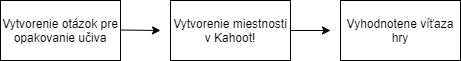
\includegraphics[scale=1.0]{diagram.pdf}
%\caption{Rozhodujúci argument.}
%\label{f:rozhod}
%\end{figure*}
\section{Kahoot!} \label{ina}
Ako som už vyššie spomínal Kahoot! je vzdelávacia platforma založená na hre. Používa sa ako vzdelávacia technológia na školách alebo na iných vzdelávacích inštitúciách v rámci game-based learningu. Kahoot! oficiálne spustili v roku 2013 za účelom aby vypomáhala učiteľom pri kreatívnejšom učení a aby viac študentov malo záujem o dané učivo.  Aplikáciu Kahoot! používa mesačne už viac ako 70 miliónov aktívnych používateľov po celom svete[3]. Toto číslo bude ale určite narastať, lebo tento typ aplikácii naberá v poslednej dobe na trende.  Popularitu aplikácie Kahoot! zapríčiňuje najmä to, že ponúka až 4 rôzne typy hier:
\begin{itemize}
\item	Kvíz
\item	Puzzle
\item	Doplňovačka
\item	Diskusia


\end {itemize}
\subsection{Ako prebieha výučba v Kahoot!} \label{ina:nejake}

Použitie aplikácie Kahoot! počas vyučovacej hodiny je ľahké, najmä preto ako jednoducho je postavená aplikácia. Učiteľ môže po vysvetlení učiva študentom vytvoriť hru v Kahoot!, kde si vyberie jednu zo 4 možností, ktorá mu pre daný moment pasuje najviac, napríklad ak chce aby si študenti preopakovali učivo, tak si zvolí kvíz. V kvíze potom vytvorí otázky a vytvorí aj kľúč správnych odpovedí. Potom ako už je kvíz vytvorený učiteľ dostane pin kód, ktorý povie svojim žiakom, vďaka ktorému sa budú môcť napojiť a zaručí to, že sa budú môcť napojiť len študenti, ktorí sú na hodine. Učiteľ sa môže rozhodnúť v aplikácii, či chce aby boli vytvorené tímy, alebo aby bol každý individuálne. Študenti potom čo sa napoja si môžu napísať svoje meno, ale pokojne môžu aj napísať čokoľvek iné v rámci zachovania anonymity odpovede.  počas kvízu. Po skončení hry, aplikácia vyhodnotí kto nazbieral najviac správnych odpovedí a stane sa víťazom, učiteľ potom môže vytvoriť ďalší kvíz alebo zvoliť iný typ hry. Na obrázku 1 môžeme vidieť ako vyzerá prostredie aplikácie Kahoot!.jkj
\begin{figure} %obrázok
\centering
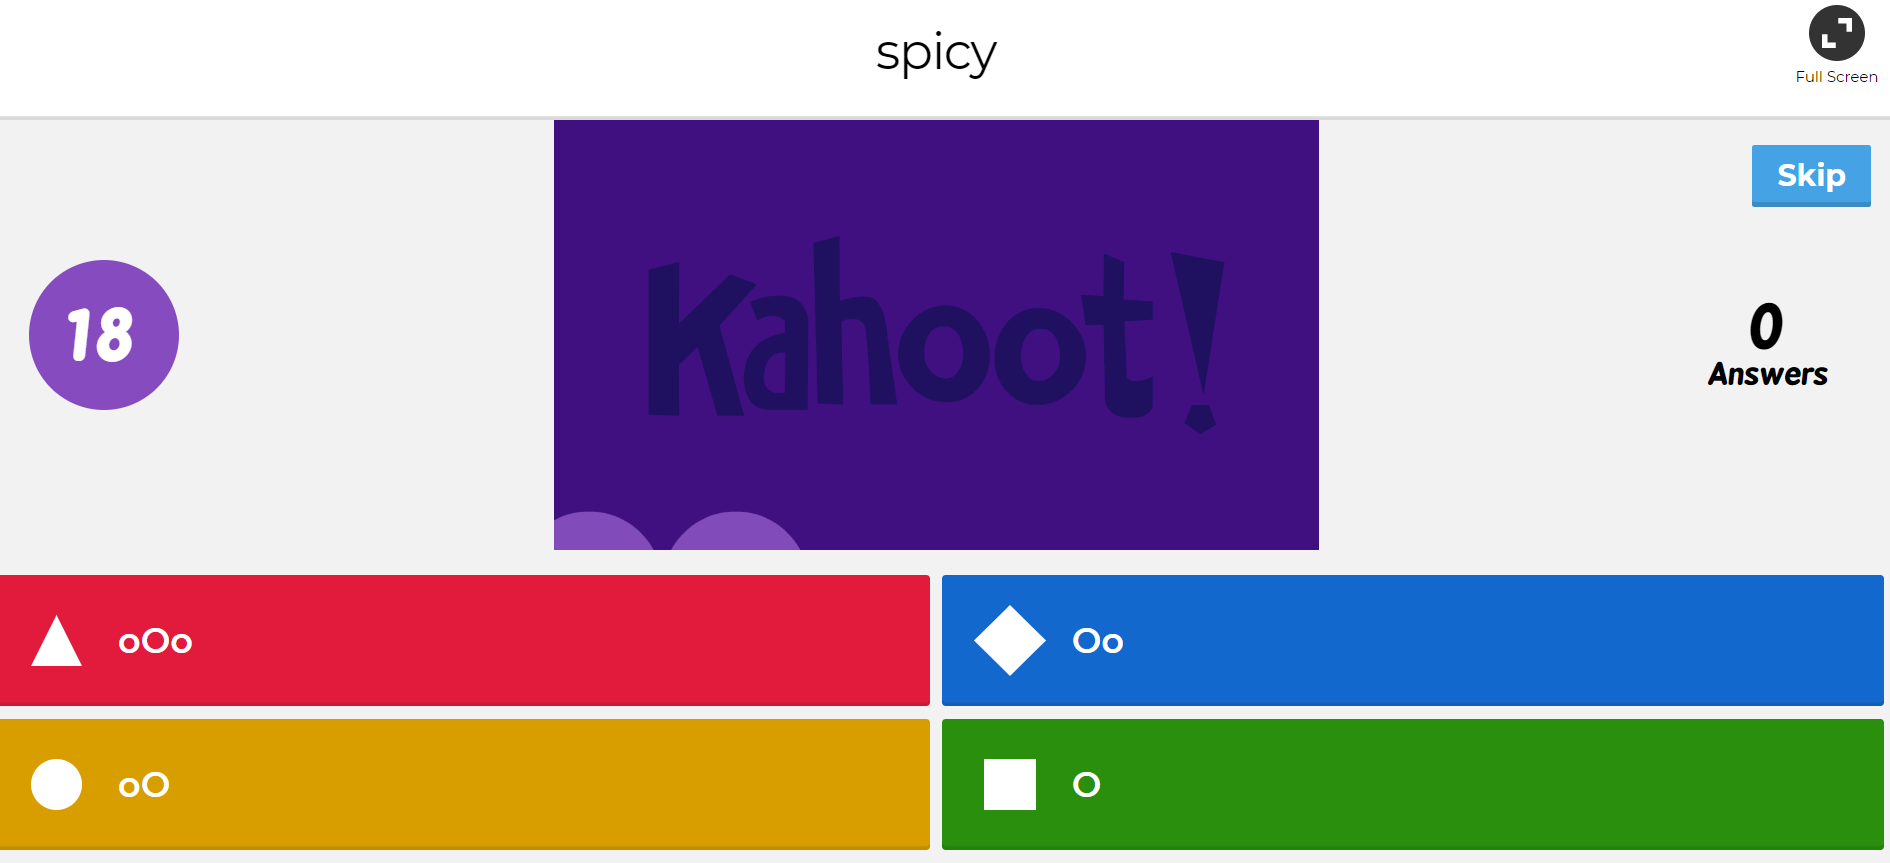
\includegraphics[width=\textwidth]{Kahoot.png}
\caption{Kahoot! počas používania kvízu}
\label{duo-uzivatelia}
\end{figure}


\subsection{Výhody a nevýhody Kahoot!} \label{ina:este}

\paragraph{Veľmi dôležitá poznámka.}
Niekedy je potrebné nadpisom označiť odsek. Text pokračuje hneď za nadpisom.



\section{1. štúdia} \label{dolezita}




\section{2. štúdia} \label{dolezitejsia}




\section{Záver} \label{zaver} % prípadne iný variant názvu



%\acknowledgement{Ak niekomu chcete poďakovať\ldots}


% týmto sa generuje zoznam literatúry z obsahu súboru literatura.bib podľa toho, na čo sa v článku odkazujete
\bibliography{literatura}
\bibliographystyle{plain} % prípadne alpha, abbrv alebo hociktorý iný

\end{document}
=======
\end{document}
>>>>>>> 298a0562592e45ba4da56c05b112c56b65884fd4
